\section{Préparer la console}
\label{sec:preparer_la_console}

Nous partirons d'ici d'un show nouvellement crée. Il est possible de créer un show
depuis l'onglet \textit{Backup}.

\subsection{Configurer les sorties}
\label{subsec:prep_sorties}

Par défaut, les sorties physiques de la console sont activées. Les ports DMX A à D sont associés aux univers 1 à 4.
Si vous utilisez un node ArtNet, il faut bien penser à activer le protocole sur la console (\textit{Setup} $\rightarrow$ \textit{Input / Output} $\rightarrow$ \textit{Enable ArtNet}).
Par ailleurs, il faut bien que la console et le node soient sur le même réseau. Il faut donc regler leurs adresse IP en conséquence (\textit{Setup} $\rightarrow$ \textit{Network Settings}).
\newline
Si vous utilisez un visualisateur comme Capture ou Wysiwyg (qui communique en Art-Net), il faut aussi regler l'adresse IP de l'ordinateur sur lequel tourne le visualisateur.

\subsection{Patch}
\label{subsec:prep_patch}

A présent, il faut ajouter les projecteurs à la console. Pour cela, il faut se rendre dans la fenetre \textit{Setup} $\rightarrow$ \textit{Patch}.
\newline
Appuyez sur \textit{Add Fixture} pour ajouter un projecteur. Vous pouvez ensuite choisir le projecteur et son mode dans la liste des fixtures disponibles (\textit{Add Type from Factory Library}).
Si le projecteur ou le mode n'est pas dans la liste, vous pouvez le créer manuellement, voir section \ref{subsec:fixture_patch}.
\newline
Les sorties d'un gradateur sont généralement patchées comme plusieurs \textit{Generic Dimmer}.
\newline
\newline
Une fois le type séléctionné, vous pouvez entrer le nombre de fixtures de ce type qui sont présentes dans votre installation.
\newline
Vous pouvez maintenant choisir l'univers sur lesquelles vous voulez les mettre, et l'adresse de départ.
Si vos projecteurs sont sur plusieurs univers differents, pas de panique, vous pouvez réajuster l'univers et l'adresse une fois les fixtures ajoutées.
\newline
Avant d'ajouter un autre type de fixture, veillez bien à regler les ID et adresses de chaque fixture déjà ajoutée en suivant ce que vous avez fait dans les sections \ref{subsec:patch_id} et \ref{subsec:patch_adressage}.
\newline
Vous pouvez ensuite faire de même pour toutes les fixtures de votre installation.
\newline
\newline
Si certaines fixtures ne sont pas présentes dans la bibliothèque du visualisateur, patchez les quand même, et effectuez les operations de ce manuel "à l'aveugle".
Referez vous ensuite à la section \ref{subsec:fixture_morph} pour pouvoir les visualiser.
\newline
\newline
\textbf{Exemple}
\newline
\newline
Mon plan de feu comporte deux ponts. Le pont de contre contient 4 Dinos et 4 Modenas qui seront sur l'univers 1.
Le pont de face contient 4 Dinos et 4 Modenas qui seront sur l'univers 2, ainsi que 4 PC1000 branchés sur les prises 1 et 3 du gradateur.
Le gradateur est branché seul sur l'univers 3.
\newline
Mon patch sur la console sera donc le suivant :
\begin{figure}[H]
    \centering
    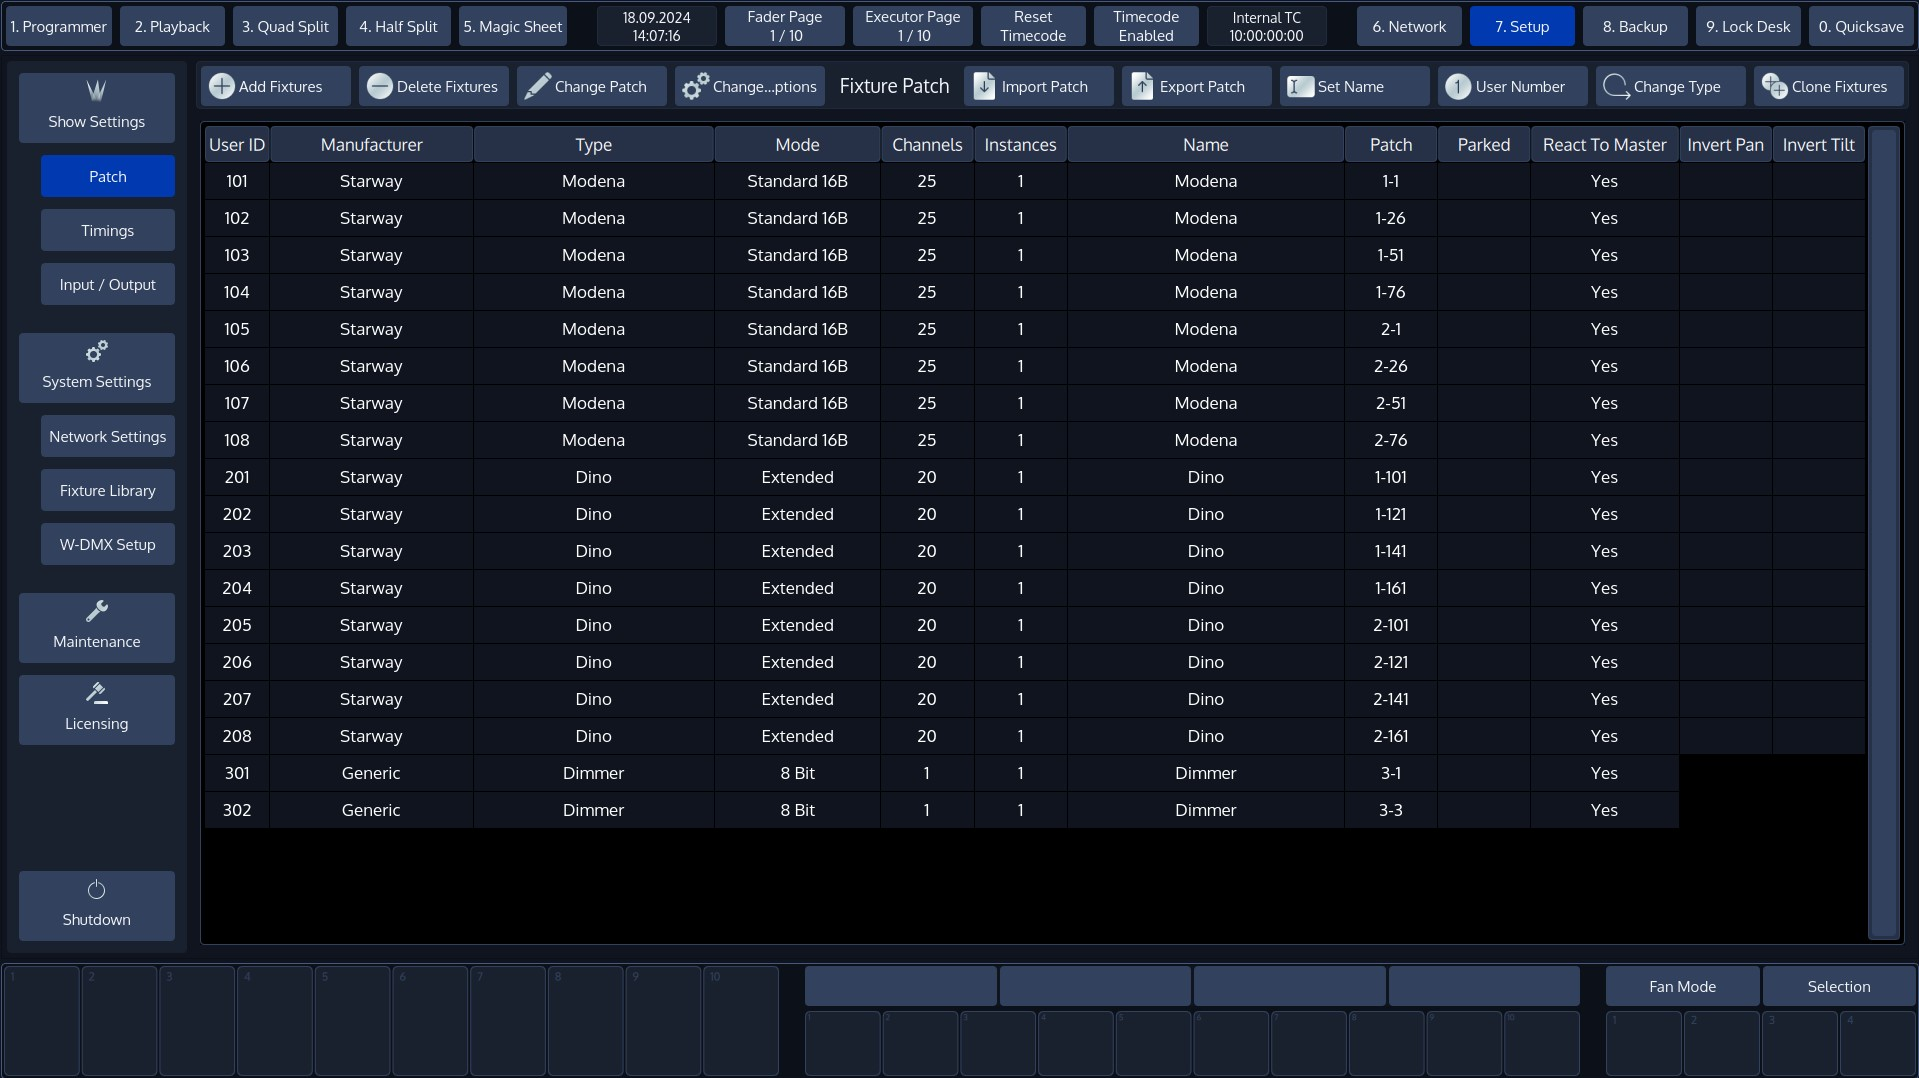
\includegraphics[width=\textwidth]{3 - Encoder la Chimp/Images/patch.jpg}
    \caption{Exemple de patch pour le plan de feu décrit}
    \label{fig:exemple_patch}
\end{figure}

\subsection{Pan/Tilt Invert}
\label{subsec:prep_invert}

Selectionnez toutes vos fixtures, allumez les et faites bouger le tilt.
Si certaines fixtures bougent dans le sens inverse d'autres, il faut activer l'inversion du tilt sur ces projecteurs.
Une fois le tilt fait, mettez les à 45° vers vous et faites bouger le pan.
Si certaines fixtures bougent dans le sens inverse d'autres, il faut activer l'inversion du pan sur ces projecteurs.
\newline
\newline
A présent, toutes vos fixtures devraient bouger dans le même sens.

\subsection{Instances}
\label{subsec:prep_instances}

Certaines fixtures, dans certains modes, peuvent comporter plusieurs \textit{instances}. Cela signifie que plusieurs parties d'une même fixture peuvent être contrôlées indépendamment.
\newline
Par exemple, une Modena en mode Pixel16B (69 canaux) comporte 8 instance.
\begin{list}{-}{}
    \item Pan/Tilt, Dimmer général, Zoom, Control, etc.
    \item LED 1 (Couleur, Dimmer et Shutter)
    \item \dots
    \item LED 7 (Couleur, Dimmer et Shutter)
\end{list}

\subsection{Colorer les fixtures}
\label{subsec:prep_colorer}

Pour faciliter la lecture des informations à l'ecran, il peut etre interessant d'associer une couleur à chaque type de fixture.
Par exemple, les Dinos seront en vert, les Modenas en Magenta et les PC1000 en jaune.
\newline
Pour cela, il faut se rendre dans la fenetre \textit{Programmer} et ouvrir une page \textit{Fixtures}.
\newline
Vous pouvez à présent voir toutes vos fixtures. Pour chacune d'entre elles, appuyez deux fois sur la touche \textit{Name} du clavier
et cliquez sur la fixture. Vous pouvez alors choisir une couleur pour cette fixture.
\newline
Par la suite, si vous voulez colorer n'importe quel élément de l'interface, c'est la même manipulation.
\newline
\newline
\textbf{Exemple}
\newline
\newline
Voici le resultat de la coloration pour mon exemple sur la figure suivante :
\begin{figure}[H]
    \centering
    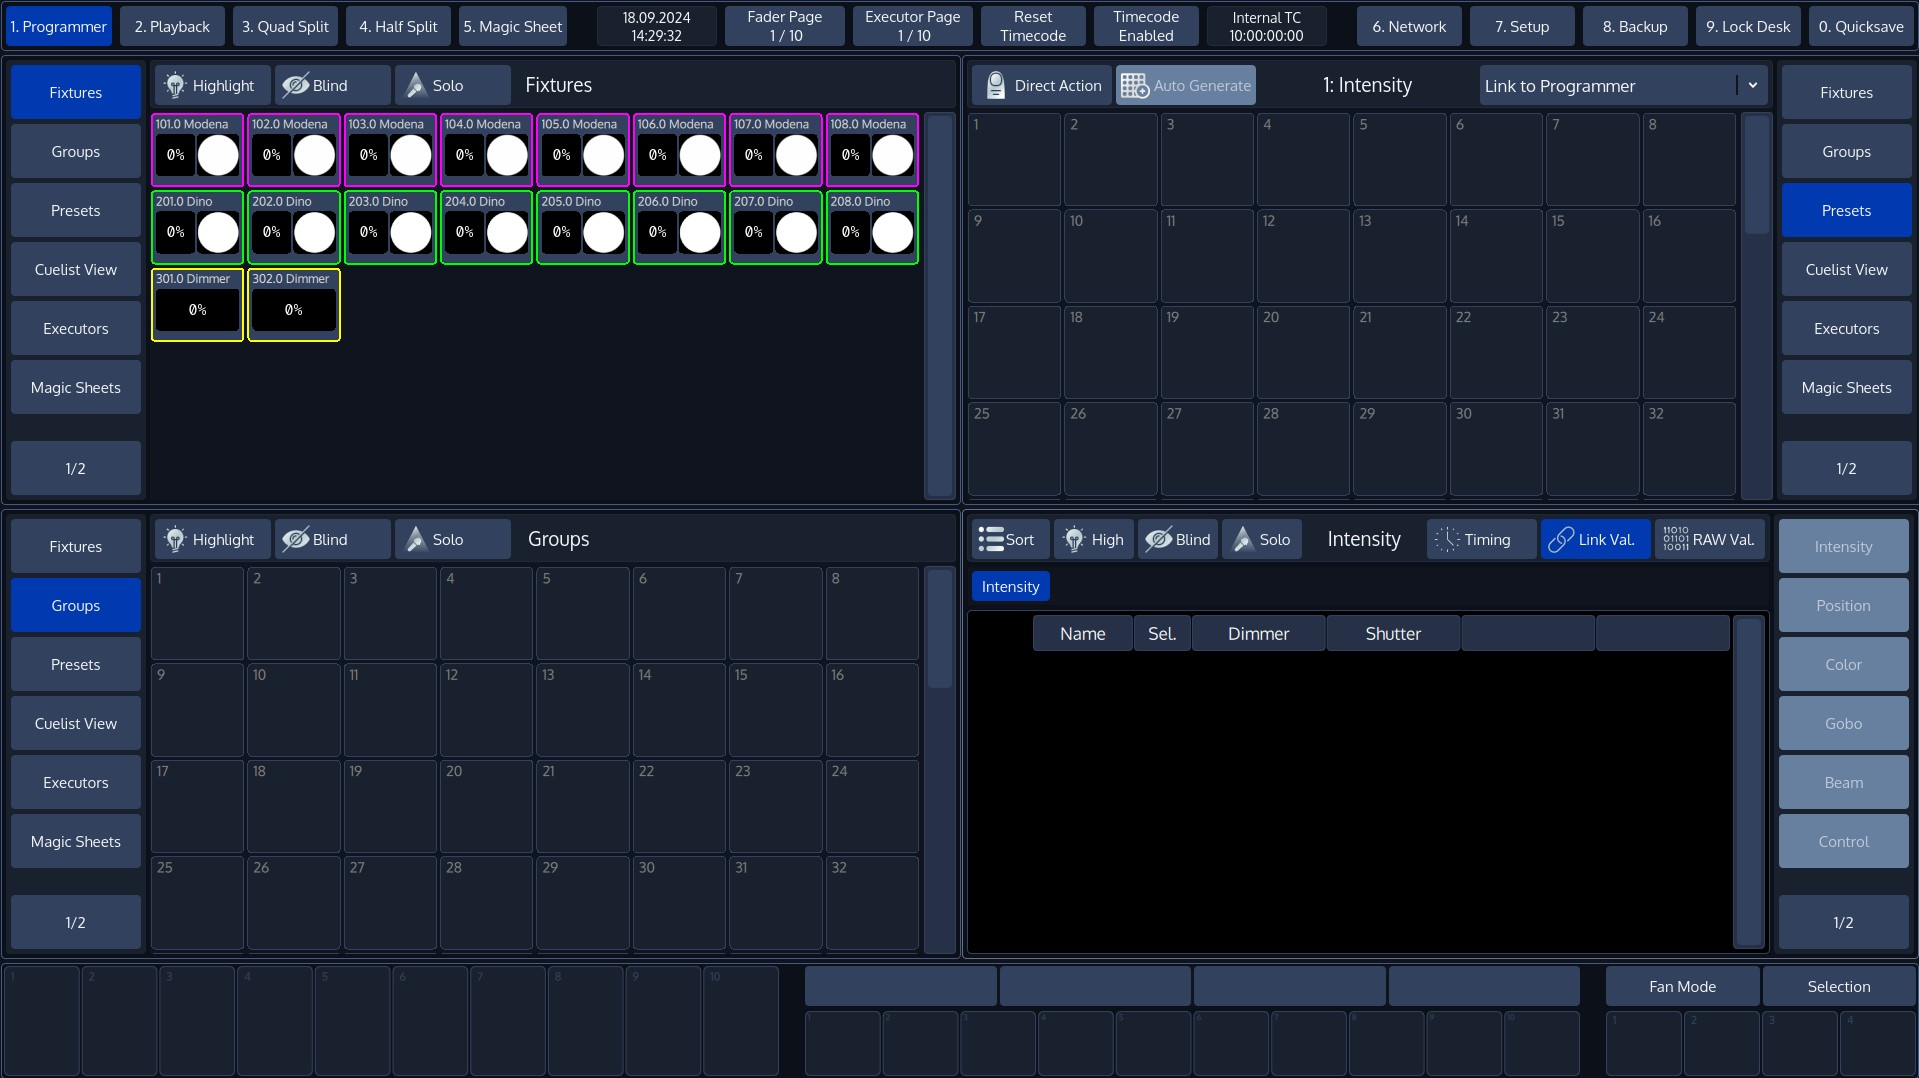
\includegraphics[width=\textwidth]{3 - Encoder la Chimp/Images/fixture_color.jpg}
    \caption{Exemple de coloration des fixtures}
    \label{fig:exemple_color}
\end{figure}

\subsection{Magic Sheet}
\label{subsec:prep_magic_sheet}

La Magic Sheet n'est pas essentielle sur les petites installations, mais elle peut tout de même faire gagner du temps.
Sur les plus grosses scènes, elle est presque indispensable.
\newline
La Magic Sheet est une page personnalisable dans laquelle on peut placer des fixtures ou des groupes de fixtures librement.
\newline
L'idée est alors de faire une page qui représente le plan de feu, avec les fixtures à leur place.
Ainsi, pas besoin de connaitre les ID par coeur pour selectionner une fixture en particulier, is suffir de la chercher dans la Magic Sheet.
\newline
\newline
Pour créer une Magic Sheet, il faut se rendre dans la fenetre \textit{Magic Sheet}, selectionner en haut a droite la page sur laquelle on veut travailler,
et appuyer sur le bouton \textit{Crayon} en haut a gauche.
\newline
On peut ensuite cliquer sur \textit{Add ...} $\rightarrow$ \textit{Fixtures} pour ajouter des fixtures à la page.
\newline
Il est maintenant possible de déplacer les fixtures sur la page.
\newline
\newline
Une fois l'opération, on peut quitter le mode édition en appuyant sur le bouton \textit{Crayon} en haut a gauche.
\newline
En revenant dans le programmer, vous pouvez remplacer la fenetre \textit{Fixtures} par la fenetre \textit{Magic Sheets} pour voir les fixtures à leur place.
\newline
\newline
Pro tip : Pour les fixtures possedant plusieurs instances comme les sunstrip (10!), la Magic Sheet peut vite devenir illisible.
Il donc est possible de regrouper les instances dans un groupe de fixtures (voir section suivante), et de mettre ce groupe dans la Magic Sheet.
\newline
\newline
\textbf{Exemple}
\newline
\newline
Voici un exemple de Magic Sheet pour mon exemple :
\begin{figure}[H]
    \centering
    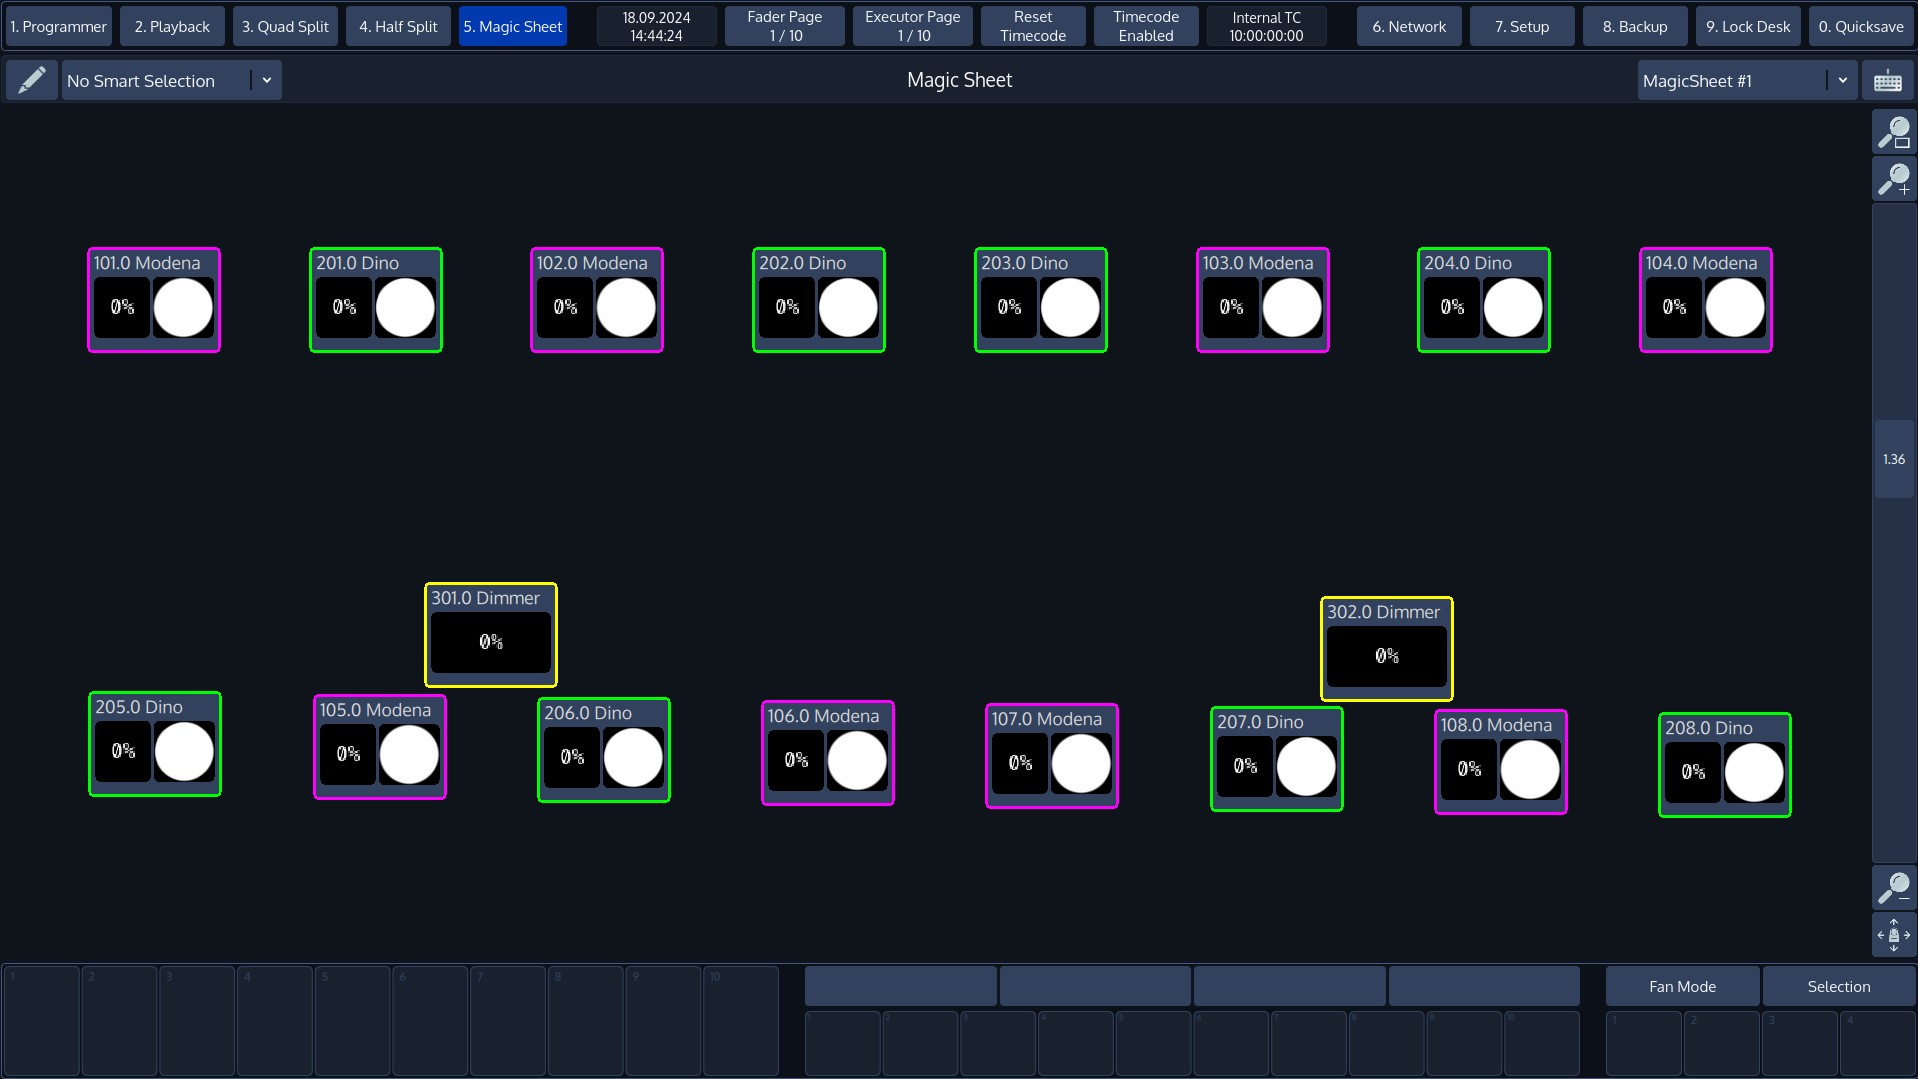
\includegraphics[width=\textwidth]{3 - Encoder la Chimp/Images/magic_sheet.jpg}
    \caption{Exemple de Magic Sheet pour le plan de feu décrit}
    \label{fig:exemple_magic_sheet}
\end{figure}

\subsection{Groupes}
\label{subsec:prep_groupes}

Les groupes permettent de regrouper des fixtures pour les manipuler plus facilement.
\newline
Il est important de noter que les groupes enregistrent l'ordre dans lequel les fixtures ont été selectionnées.
Cela va s'averer important pour la création d'effets (voir section \ref{subsec:exec_effets}).
\newline
\newline
Pour créer un groupe, il faut se rendre dans la fenetre \textit{Programmer} et ouvrir une page \textit{Groups}
(elle est ouverte par defaut dans la fenetre en bas à gauche).
\newline
Selectionnez ensuite les fixtures que vous voulez regrouper dans un ordre interessant (depuis la Magic Sheet ou la page Fixtures), appuyez sur la touche \textit{Rec} du clavier et cliquez sur une case vide de la fenetre de groupe.
Donnez un nom au groupe qui traduit de ce qu'il contient, et l'ordre dans lequel les fixtures ont été selectionnées.
\newline
\newline
\begin{list}{-}{Ordres de selection utiles :}
    \item LTR : Left To Right. Selectionnez les fixtures de gauche à droite, peu importe le pont sur lequel elles sont.
    \item Sym : Symétrique. Selectionnez tantôt une fixture à droite, tantôt une fixture à gauche, en veillant à ne pas selectionner
deux fixtures symétriques. Une fois arrivé à la moitié, selectionnez le symétrique des fixtures déjà selectionnées, dans l'ordre inverse.
\newline
Dans mon exemple, un groupe Sym de Modenas pourrait être : 101, 107, 105, 103, 102, 108, 106 et 104.
    \item D'autres ordres peuvent être interessant, dépendant des effets que vous souhaitez faire.
\end{list}
\textbf{Exemple}
\newline
\newline
Dans mon cas, je vais créer 5 groupes : Modena LTR, Modena Sym, Dino LTR, Dino Sym et PC1000.

\subsection{Masters}
\label{subsec:prep_gm}

Pour terminer de préparer la console, il faut créer les Masters.
Le Grand Master est un fader qui permet de régler l'intensité générale de tous les projecteurs.
\newline
Pour ce faire, cliquez sur le rectangle associé au premier fader de la console~: il est noté 1 en bas à gauche.
\newline
Allez ensuite dans l'onglet \textit{Global Masters} et selectionnez le \textit{Grandmaster}.
\newline
\newline
Montez le premier fader de la console à 100\% pour que le Grand Master soit à 100\%.
\newline
\newline
Maintenant, nous allons créer les Masters de vitesse. Ils se situent au niveau des 4 faders à droite de la console.
Cliquez sur chaque carré et selectionnez dans l'ordre : FX Speed Master 1, FX Speed Master 2, Speed Master 1 et Fade Master 1.
\newline
Ils nous seront utiles plus tard.
\newline
\newline
\textbf{Exemple}
\newline
\newline
Voici l'état de la console après toutes ces opérations :
\begin{figure}[H]
    \centering
    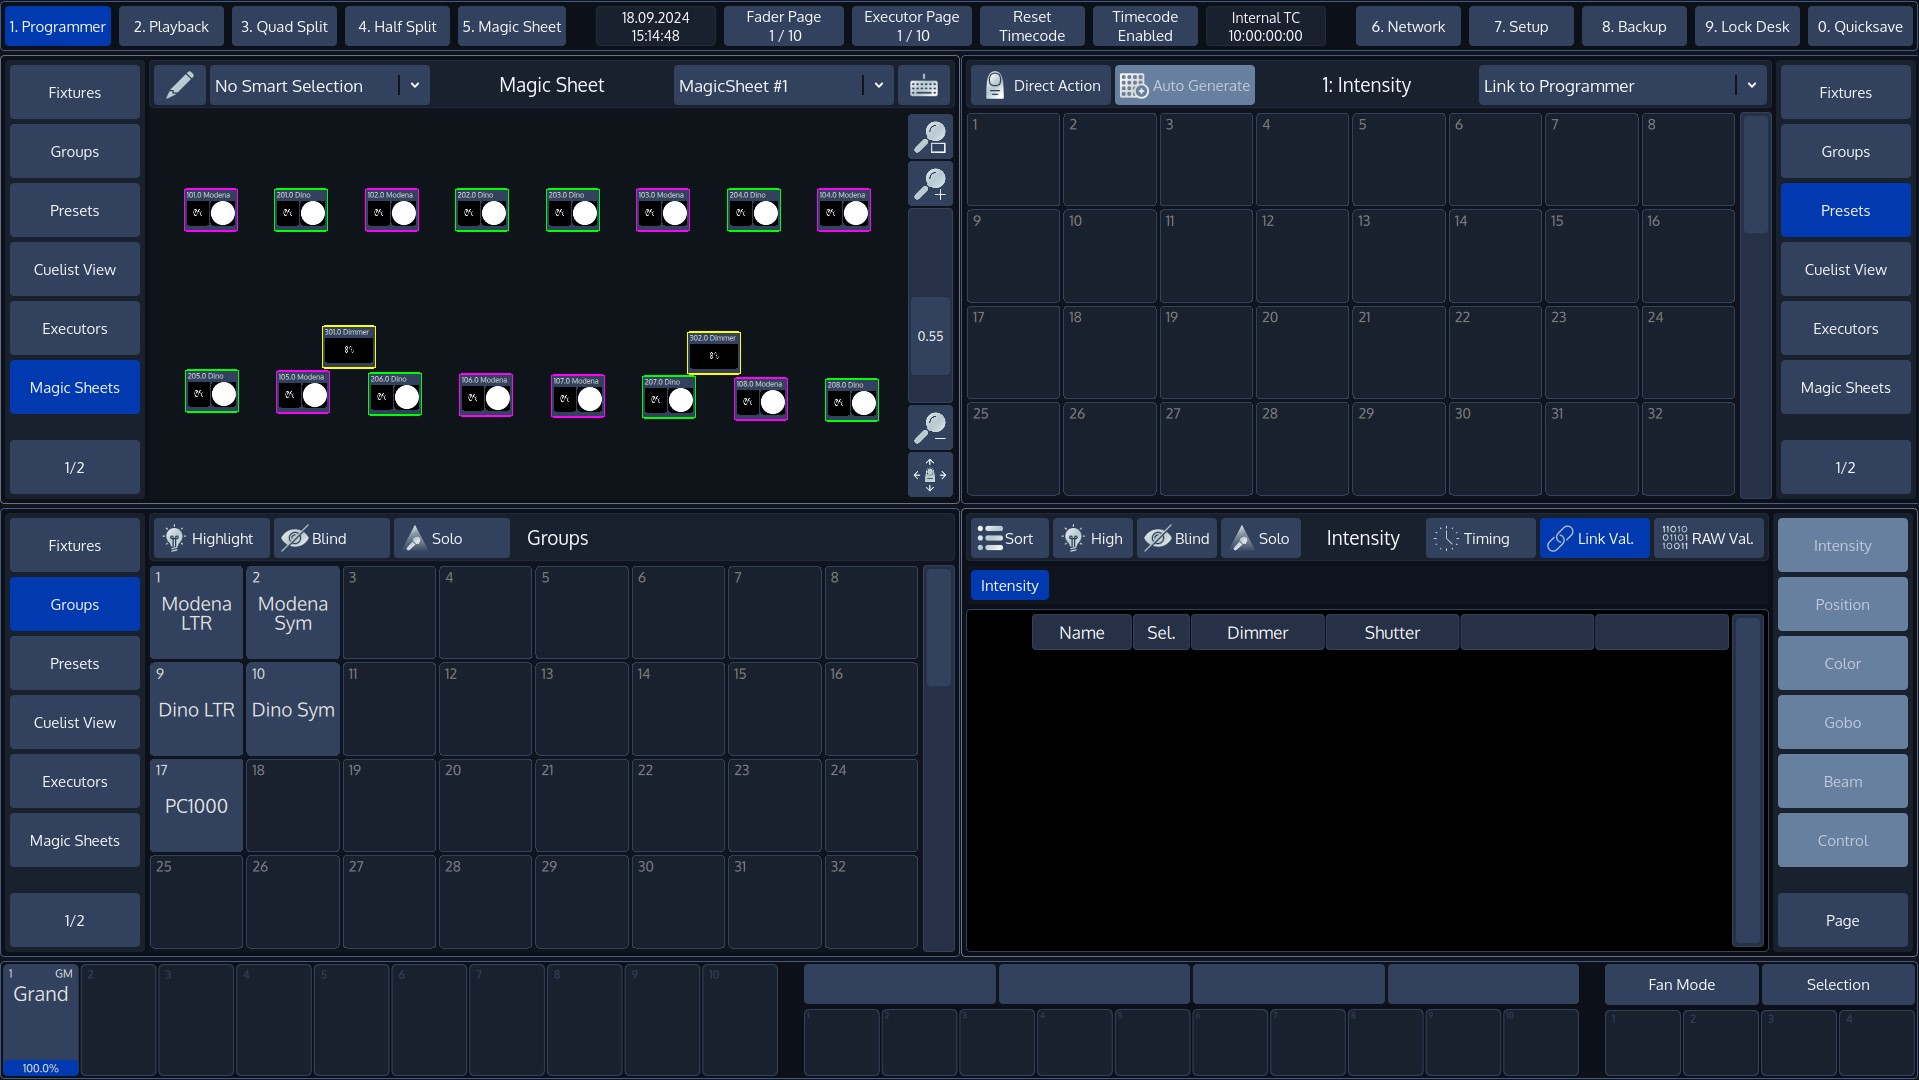
\includegraphics[width=\textwidth]{3 - Encoder la Chimp/Images/prep_final.jpg}
    \caption{Console après préparation}
    \label{fig:prep_finale}
\end{figure}
